\addcontentsline{toc}{chapter}{Summary}
%\thispagestyle{empty}

%\vspace*{20mm}
\KOMAoptions{headsepline=false}

\begin{center}
    {\usekomafont{sectioning}\usekomafont{section}\textbf{\large Summary} }
\end{center}

This project falls within an Unseen 6 \ac{DoF} competition, organized in collaboration with the \ac{ESA} Advanced Concept Team. Essentially, we are dealing with space objects that are unfamiliar to us, and our objective is to accurately predict their 6\ac{DoF} poses. The action of the \ac{CVLab} team is twofold: firstly, we are tasked with creating a challenging dataset featuring multi-object, unseen, and occluded spacecraft scenarios. This involves ensuring a high degree of rendering realism. Secondly, we are focused on developing a baseline solution, which entails implementing a pose estimation model and conducting thorough training and testing on our dataset. My role this semester was primarily concentrated on the latter aspect, specifically on a track that incorporated target models.

\bigbreak 

Foremost, we started with a literature search by reading recent papers about generalizable 6DoF object pose estimation\footnote{\url{https://github.com/liuyuan-pal/Awesome-generalizable-6D-object-pose}}. Among the various models we explored, one that particularly captured our attention was the "Generalizable Model-Free 6-DoF Object Pose Estimation from RGB Images," commonly referred to as Gen6D \cite{liu2023gen6d}. We have compiled a table summarizing the advantages and disadvantages of this architecture for a clearer understanding:

\begin{table}[htpb]
  \caption[Example table]{Summary of Gen6D}\label{tab:sample}
  \centering
  \small
  \begin{tabular}{l | l}
    \toprule
      Pros & Cons \\
    \midrule
      Generalizability & Limited by Reference Image Quality \\
      Model-Free & Everyday Life Objects Training Data \\
      Simple Input Requirements & Difficulty with Symmetric Objects \\
      Robustness to Background Clutter & Dependence on Initial Detection and Selection \\
      Effective in Diverse Environments & Potential Challenges with Severe Occlusions \\
      Competitive Performance & Computationally Intensive \\
    \bottomrule
  \end{tabular}
\end{table}

We need to point out that Gen6D does not need a model because it uses a \ac{SFM} software called \textit{Colmap}. As we are on the track with the target models included, we simply skip this reconstruction step.

\bigbreak 

After selecting the model, we needed to establish a suitable environment for executing the code: EPFL Scitas Izar servers. Equipped with two NVIDIA V100 PCIe 32 GB GPUs, these servers are ideally configured for our \ac{ML} task. However, this stage proved to be more time-consuming than expected. It entailed various technical challenges, including setting up the virtual environment, installing the necessary dependencies, composing the bash execution script, and, fundamentally, learning the correct way to utilize the server.

After resolving the engineering aspects, we were able to delve into the practical side of the project, working directly with the code to adapt it to our dataset. After understanding the code, the initial task involved developing a data loader specifically for the Spacecraft dataset. This was accompanied by various minor modifications within the code, such as updating names and adjusting data paths. To align with the data format used by Gen6D for poses, it was necessary to write a Python script. This was because our dataset utilized quaternions combined with a translation vector in one text file, whereas Gen6D's format employed a rotation matrix augmented by the translation vector formatted as a separate numpy array for each image.

\KOMAoptions{headsepline=true}

Next, we tackled the debugging phase, aimed at addressing the model's accuracy issues. We encountered several problems. For instance, we needed to rectify the inverted masks for the objects using a Python script with the OpenCV library. Additionally, the model processes the reference images by cropping them into 128x128 pixel dimensions, while the detector is designed to identify objects in the query images that range from half to double the size of the reference images. Consequently, we resized the query images to reduce the scale difference relative to the reference images. This resizing was accompanied by necessary adjustments to the intrinsic matrix. Also we had to enhance the selection process of the reference images to ensure a more uniform distribution around the objects: contrary to everyday objects, spacecrafts can be observed from any angle, this should be considered in our approach.

\bigbreak 

One should bear in mind that in this model implementation, we decided to not retrain Gen6D. As a result, the outcomes are now more reliant than ever on the quality of the reference images. Given that we have access to highly realistic renderings of the spacecrafts and precise ground truth poses provided by the dataset team, we aim to assess Gen6D's effectiveness across a range of objects. Below are the visual results for the Hubble object:

\begin{figure}[ht]
  \centering
  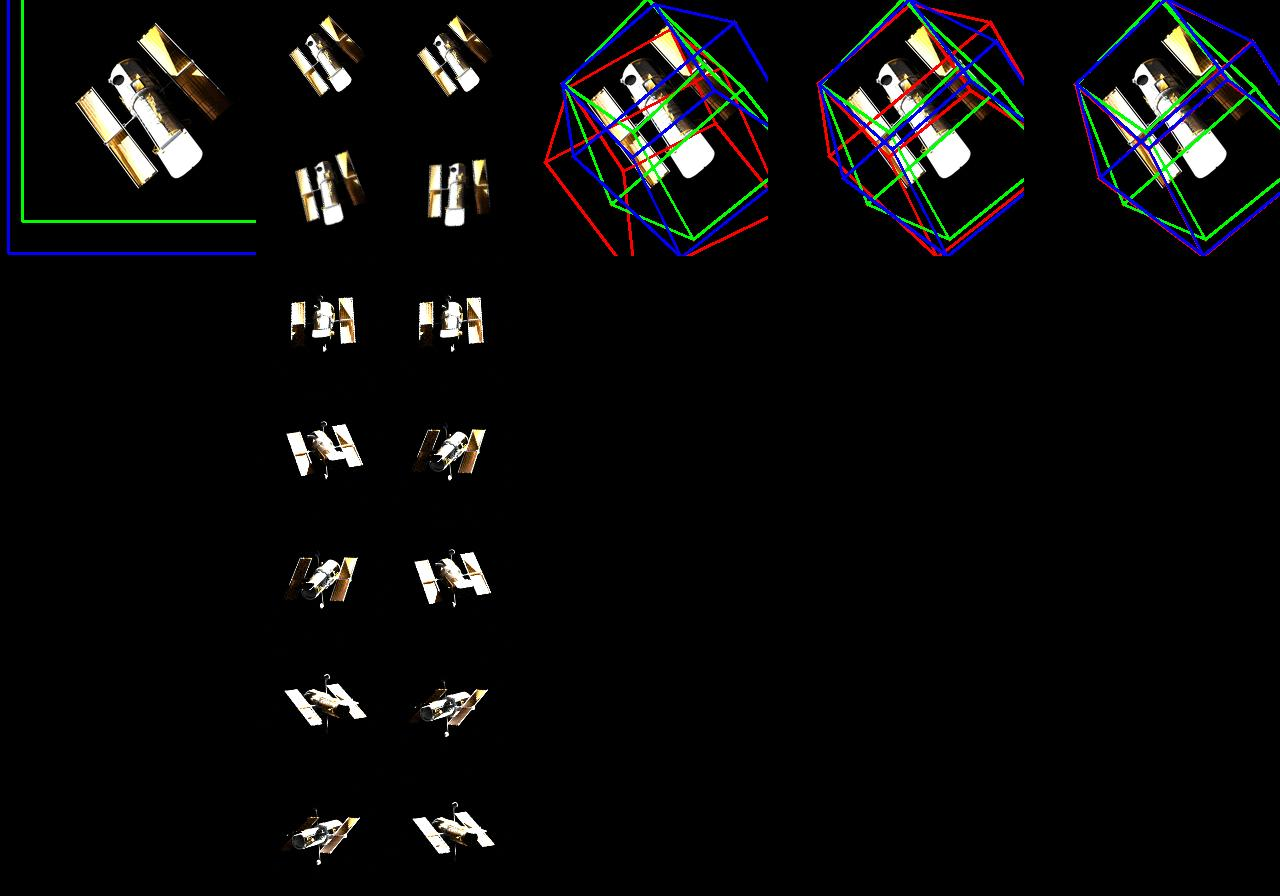
\includegraphics[width=\textwidth]{data/res2.jpg}
  \caption{An Estimation by Gen6D (Highlighted in Blue) of the Hubble Object, Presented Without a Background.}
  \label{fig:cap1}
\end{figure}

\begin{figure}[ht]
  \centering
  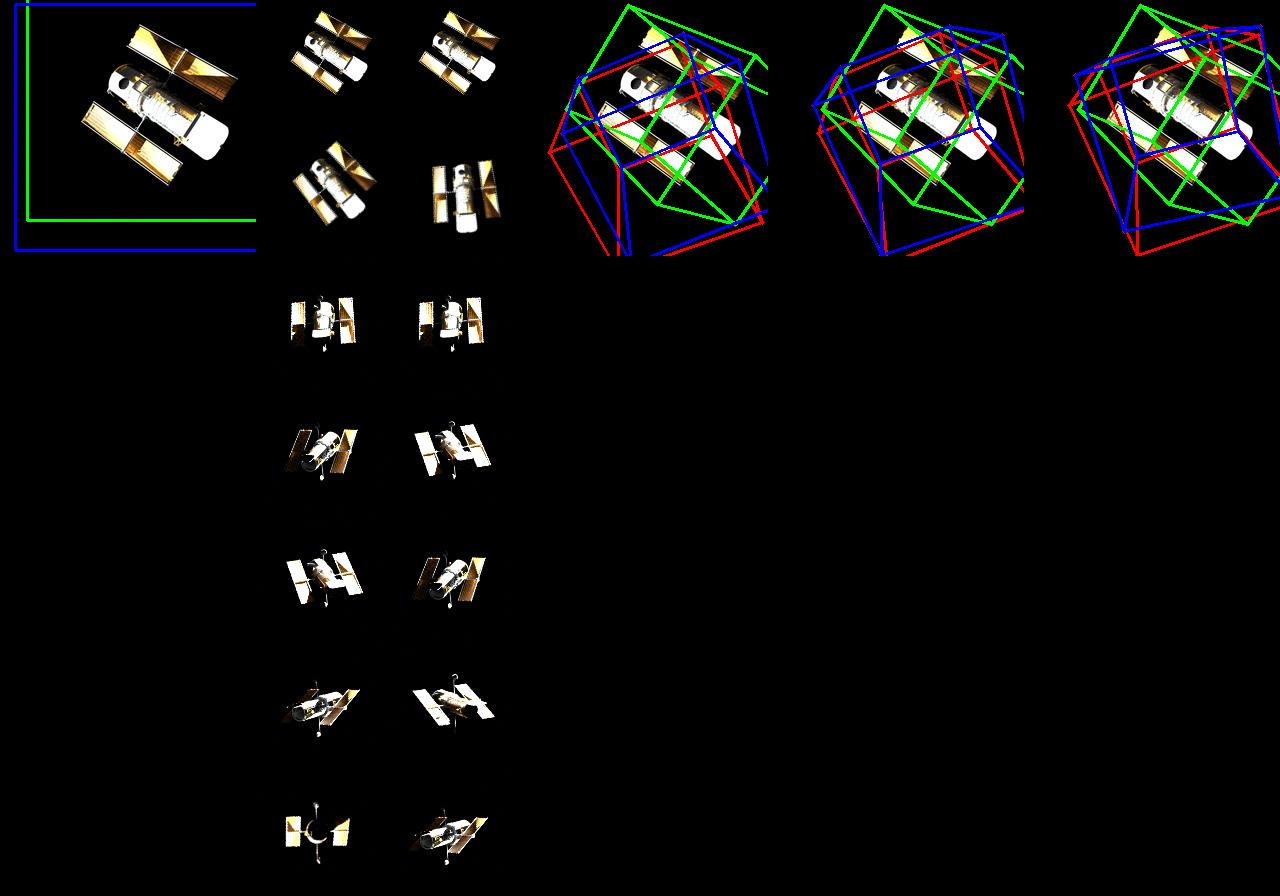
\includegraphics[width=\textwidth]{data/res3.jpg}
  \caption{An Estimation by Gen6D (Highlighted in Blue) of the Hubble Object, Presented Without a Background. Gen6D happens to lack of accuracy.}
  \label{fig:cap1}
\end{figure}

\begin{figure}[ht]
  \centering
  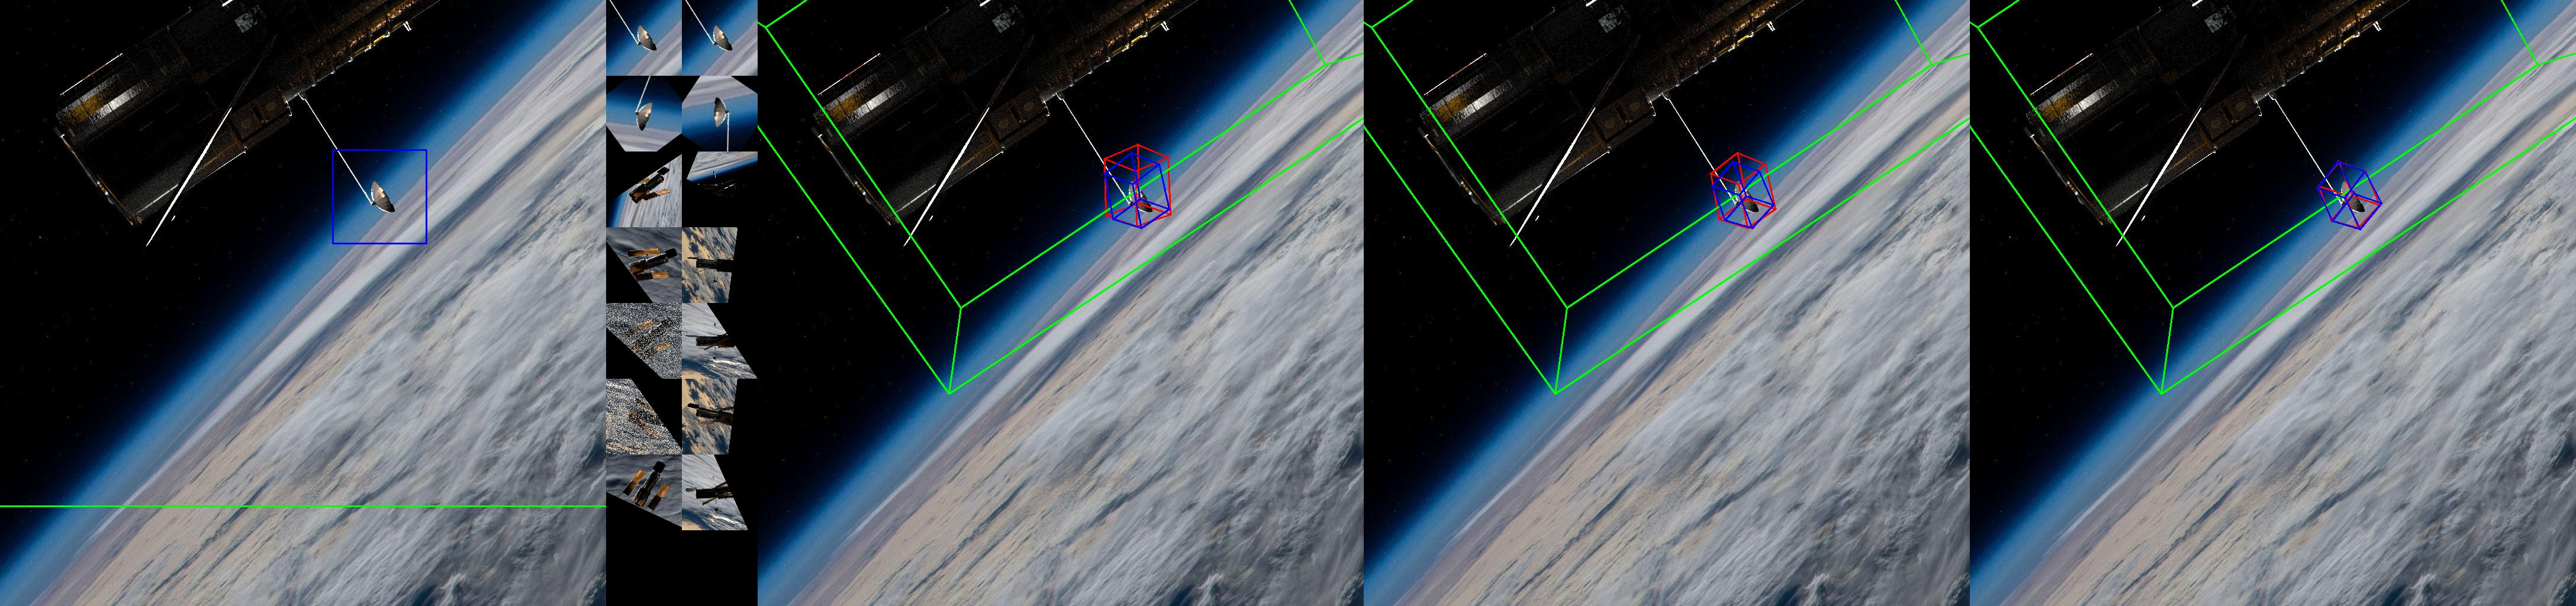
\includegraphics[width=\textwidth]{data/res4.jpg}
  \caption{An Estimation by Gen6D (Highlighted in Blue) of the Hubble Object, Presented With a Background. Here the query object size is too big for the detector.}
  \label{fig:cap4}
\end{figure}

\begin{figure}[ht]
  \centering
  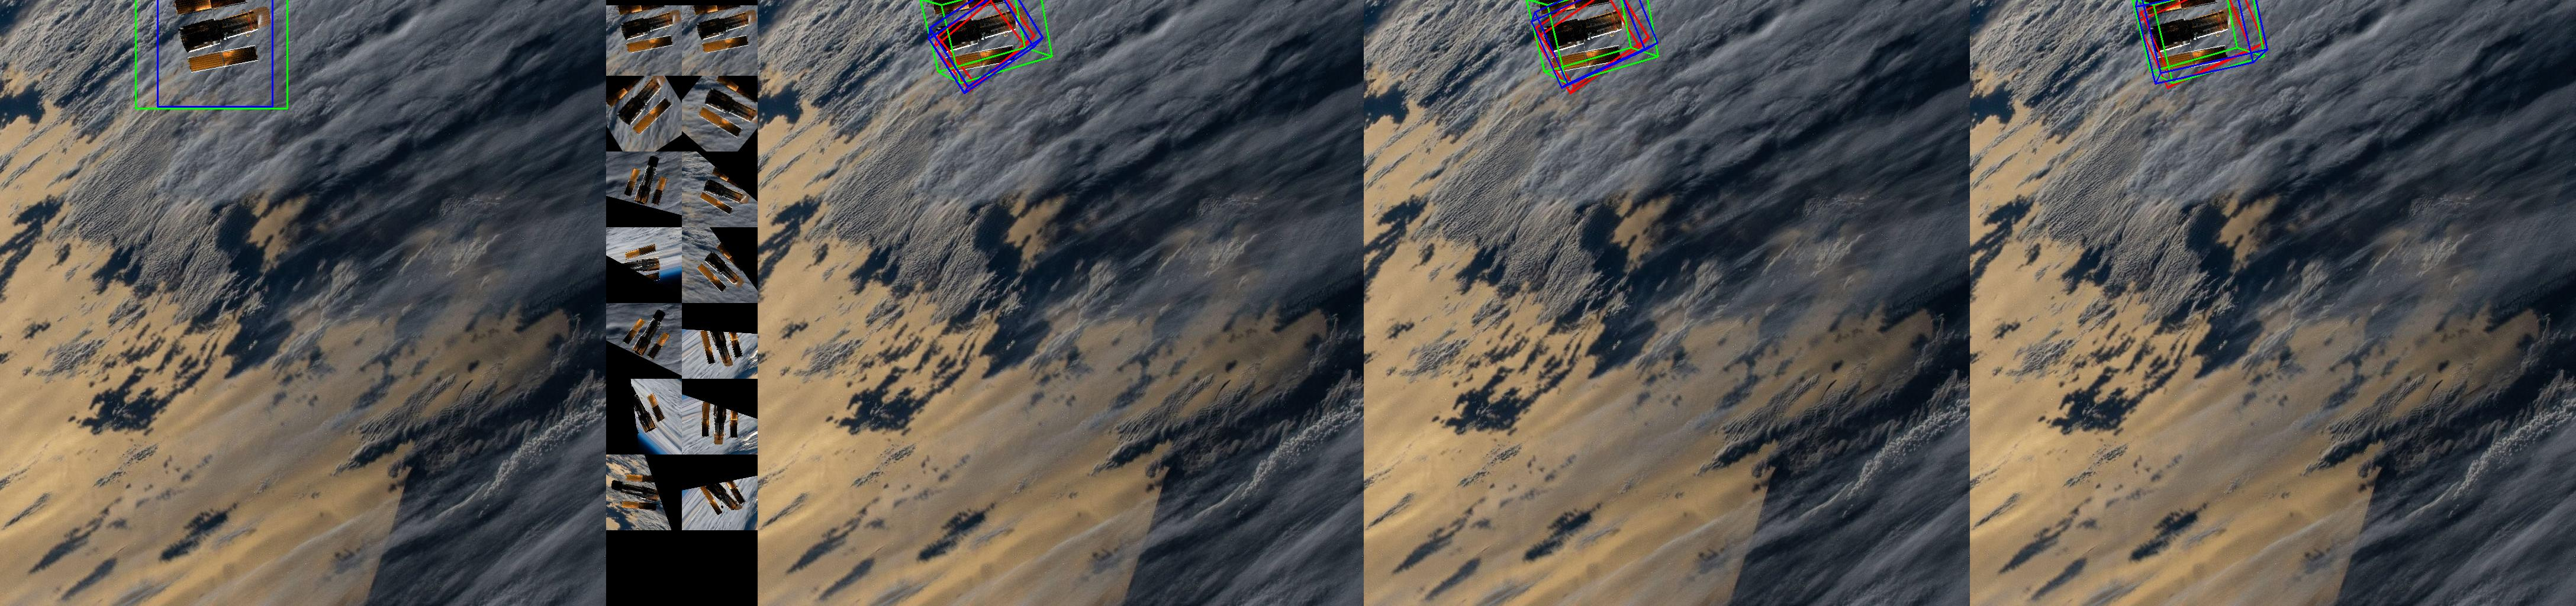
\includegraphics[width=\textwidth]{data/res1.jpg}
  \caption{An Estimation by Gen6D (Highlighted in Blue) of the Hubble Object, Presented With a Background.}
  \label{fig:cap2}
\end{figure}



